\documentclass[conference, letterpaper]{IEEEtran}

\usepackage[T1]{fontenc}
\usepackage[utf8]{inputenc}
\hyphenation{op-tical net-works semi-conduc-tor}

\ifCLASSINFOpdf
   \usepackage[pdftex]{graphicx}
\else
\fi

\usepackage[cmex10]{amsmath}
\usepackage{amssymb}
\usepackage{color}
\usepackage{flushend}
\usepackage{fancyhdr}
\usepackage{subcaption}
\usepackage{balance}
\captionsetup[table]{justification=centering, labelsep=period, font={footnotesize,sc}}
\captionsetup[figure]{justification=centering, labelsep=period, font={footnotesize}}
\usepackage{booktabs}
\usepackage{algorithm}
\usepackage{algpseudocode}
\usepackage{threeparttable}
\usepackage{xcolor}
\usepackage{url}
\usepackage{hyperref}

\graphicspath{{../results/figures/}}

\renewcommand{\thispagestyle}[2]{}

\fancypagestyle{plain}{
        \fancyhead{}
        \fancyhead[C]{first page center header}
        \fancyfoot{}
        \fancyfoot[C]{first page center footer}
}
\pagestyle{fancy}

\headheight 20pt
\footskip 20pt

\rhead{}

\setcounter{page}{1}

\fancyhead[R]{\textit{(IJACSA) International Journal of Advanced Computer Science and Applications, \\ Vol. XXX, No. XXX, 2026}}
\renewcommand{\headrulewidth}{0pt}

\fancyfoot[C]{www.ijacsa.thesai.org}
\renewcommand{\footrulewidth}{0.5pt}
\fancyfoot[R]{\thepage \  $|$ P a g e }

\begin{document}

\title{Metaheuristic Co-Optimization of Compression and Runtime Configuration for Embedded LLM Inference: A Case Study on TinyLlama and Raspberry Pi 5}

\author{
\IEEEauthorblockN{Fahd Koraiche\IEEEauthorrefmark{1}\footnotemark[1], Rachid Dehbi\IEEEauthorrefmark{1}, Amine Dehbi\IEEEauthorrefmark{2}}
\IEEEauthorblockA{\IEEEauthorrefmark{1}Research Laboratory of Data Engineering and Intelligent Systems (LIDSI), Faculty of Science A\"{i}n Chock, Casablanca, Morocco\\
\IEEEauthorrefmark{2}Research Laboratory of Mathematics and Computer Science (LTI), Faculty of Sciences Ben M'Sik, Casablanca, Morocco;\\
High School of Technology-Dakhla, Dakhla, Morocco}
}

\maketitle
\renewcommand{\thefootnote}{\fnsymbol{footnote}}
\footnotetext[1]{Corresponding author (fahd.koraiche@gmail.com)}

\begin{abstract}
Deploying large language models (LLMs) on resource-constrained edge devices requires navigating a large, mixed discrete-continuous configuration space spanning model compression and inference runtime settings. This paper formulates embedded LLM deployment as a two-phase optimization problem: an exhaustive discrete phase over quantization variants, followed by a continuous/combinatorial metaheuristic search over runtime parameters. We validate three metaheuristics---particle swarm optimization (PSO), grey wolf optimizer (GWO), and differential evolution (DE)---on standard benchmark functions, then apply them, with full hardware-in-the-loop measurement (latency, memory, on-device energy via the target board's power-management IC, and perplexity), to tune TinyLlama-1.1B inference across all seven Pareto-nondominated quantization variants identified by an exhaustive Phase 1 sweep, on a Raspberry Pi 5. Phase 2 surfaces a finding beyond simple algorithm comparison: systematically cross-checking every reported ``best'' configuration's scalarized cost against an independent re-measurement of that same configuration reveals the optimizer's curse---population-based metaheuristics' iterative convergence toward a promising region repeatedly samples nearby noisy real-hardware measurements, so the single lowest cost recorded during a run is a biased, overly optimistic estimator of that configuration's true cost. This effect ranges from negligible (several variants' results reconcile to within 33\%) to severe (one variant's best-appearing result is 61 times more optimistic than an independent re-measurement supports), and on two of the seven variants it is severe enough that a naive baseline (grid or random search) outright beats every metaheuristic once the noise-corrupted results are excluded. A hardened follow-up experiment, adding repeated measurements and independent verification before reporting any winner, confirms this is not a single-measurement artifact and surfaces a stronger result on one variant: no method, including the baselines, reconciles at all. This variance in both outcome and measurement reliability across variants---not a single clean percentage---is the paper's central finding: real per-evaluation cost, orders of magnitude above the millisecond-scale costs assumed in prior metaheuristic-tuning work, forces a small evaluation budget that is measurably more exposed to this bias than synthetic or simulator-based benchmarks.
\end{abstract}

\begin{IEEEkeywords}
Edge AI; Embedded large language models; Hyperparameter tuning; Metaheuristic optimization; Model compression; Quantization; TinyLlama
\end{IEEEkeywords}

\section{Introduction}
\label{sec:introduction}

Large language models (LLMs) are increasingly deployed outside the datacenter, on phones, microcontrollers, and single-board computers, driven by privacy, latency, connectivity, and cost concerns~\cite{ref17}. Running an LLM on a device such as the Raspberry Pi 5 (8 GB RAM, no dedicated GPU) is only feasible after aggressive compression---primarily post-training quantization---and careful runtime configuration of the inference engine (thread count, batch size, context length, KV-cache behavior). Unlike cloud deployment, where extra compute can mask a suboptimal configuration, embedded deployment operates under hard resource ceilings: a configuration that exceeds available RAM fails outright rather than degrading gracefully.

Model compression research (GPTQ~\cite{ref4}, AWQ~\cite{ref5}, LLM.int8()~\cite{ref6}, SqueezeLLM~\cite{ref7}) optimizes a quality/size trade-off independently of the serving runtime and target hardware; systems work on inference engines (e.g., llama.cpp~\cite{ref3}) exposes dozens of runtime flags but leaves their tuning to manual trial-and-error. Neither line of work treats compression choice and runtime configuration as parts of a single search problem evaluated end-to-end on the physical target device. Hyperparameter-optimization metaheuristics---PSO~\cite{ref8}, GWO~\cite{ref9}, DE~\cite{ref10}---have been shown to outperform naive grid/random search when tuning classical ML models; Nouna et al.~\cite{ref11} demonstrated this for heart disease prediction (PSO/GWO/DE tuning KNN/SVM after wrapper-based feature selection, validated on synthetic functions before the real objective), and that preprocessing$\rightarrow$validation$\rightarrow$tuning structure is the direct methodological inspiration for this work.

We adapt that structure to a fundamentally different cost regime: in~\cite{ref11}, one fitness evaluation costs milliseconds; here, evaluating one candidate runtime configuration can cost seconds to minutes on physical hardware, since it may require loading a multi-hundred-megabyte quantized model and running real generation workloads. This cost asymmetry is the central engineering constraint of our method design (Section~\ref{sec:method}): naively porting a flat metaheuristic search vector from the classical-ML setting is computationally infeasible, and the two-phase discrete/continuous decomposition we propose is what makes hardware-in-the-loop metaheuristic tuning tractable on a Raspberry Pi 5.

\textbf{Contributions:} (1) a two-phase search formulation---exhaustive discrete quantization-variant selection followed by metaheuristic runtime tuning---that makes hardware-in-the-loop optimization of embedded LLM inference tractable; (2) a multi-objective evaluation function jointly capturing quality, latency, memory, and energy per token, with hard feasibility constraints enforced by rejection rather than soft penalty; (3) an empirical comparison of PSO, GWO, and DE for this task on physical hardware, with explicit control for thermal throttling and OS jitter; (4) identification and systematic measurement of the optimizer's curse as a concrete failure mode of hardware-in-the-loop metaheuristic search, together with a comparison against grid search, random search, and baselines under an equalized evaluation budget; (5) a hardened post-experiment follow-up that tests whether repeated measurement and independent verification actually resolves the optimizer's curse.

\section{Related Work}
\label{sec:related}

Post-training quantization (GPTQ~\cite{ref4}, AWQ~\cite{ref5}, LLM.int8()~\cite{ref6}, SqueezeLLM~\cite{ref7}) reduces model size and memory bandwidth at some quality cost; TinyLlama~\cite{ref1} is trained from scratch at 1.1B parameters specifically to be inference-efficient, making it a natural target for the runtime-side compression this paper studies. llama.cpp~\cite{ref3} enables CPU-only inference on commodity edge hardware via GGUF quantization (Q2\_K--Q8\_0, Section~\ref{sec:phase1}); NPU-offloaded inference~\cite{ref18} is a complementary hardware-acceleration path to this paper's CPU-only approach. Edge-LLM survey work catalogs the broader deployment landscape~\cite{ref17}.

Grid and random search scale poorly with dimensionality; PSO~\cite{ref8}, GWO~\cite{ref9}, and DE~\cite{ref10} have been applied to tune classical ML models, most directly by~\cite{ref11} (Section~\ref{sec:introduction}). On the quantization-search side, HAQ~\cite{ref12} uses reinforcement learning (not a population-based metaheuristic) with a hardware \emph{simulator} to search per-layer CNN bitwidths; genetic-algorithm~\cite{ref13}, evolving-proxy~\cite{ref14}, and bare-bones-PSO~\cite{ref15} methods search CNN quantization directly but target CNNs, search quantization alone, and evaluate via simulators/GPUs rather than a physical low-power board. LLM-guided PSO~\cite{ref16} uses an LLM \emph{inside} the optimizer to tune conventional DL hyperparameters---a different problem from this paper's PSO/GWO/DE tuning an LLM's own deployment configuration.

\textbf{The closest prior art is LLMPi}~\cite{ref19} (physical-Raspberry-Pi LLM quantization measurement, but fixed quantization levels, no metaheuristic search, no runtime-configuration search) and \textbf{DeepQGHO}~\cite{ref20} (physical Jetson Nano, joint hyperparameter search plus quantization, but greedy coordinate descent on training-time CNN hyperparameters, quantized only after search completes). Two 2026 studies narrow the gap further without closing it: Embedded Arena~\cite{ref21} co-optimizes MCU model/firmware via an LLM-agent (not population-based) on vision/audio targets (not LLM inference); Sadheerthan et al.~\cite{ref22} use PSO to design a TinyLlama softmax approximation measured on a physical NPU, but search one kernel's design rather than compression plus serving-runtime configuration, without end-to-end LLM latency. Based on four targeted search passes, no located work combines (a) a population-based metaheuristic, (b) joint LLM compression and runtime-configuration search, (c) physical low-power hardware-in-the-loop measurement, and (d) LLM inference as the target; this is an evidence-based gap, not an unqualified ``first'' claim (Section~\ref{sec:limitations}).

\section{Method}
\label{sec:method}

\subsection{Two-Phase Decomposition}
We decompose the search space into two tiers, mirroring~\cite{ref11}'s preprocessing/feature-selection $\rightarrow$ hyperparameter-tuning structure (Fig.~\ref{fig:pipeline}): \textbf{Phase 1} (discrete, exhaustive) selects a quantization variant from a small catalog; \textbf{Phase 2} (metaheuristic) tunes continuous/combinatorial runtime parameters for the chosen variant using PSO, GWO, and DE. This split exists because quantization variants are distinct requantized model artifacts, not continuously interpolable, while runtime parameters can be varied on a fixed model file at near-zero marginal cost---flattening both into one search vector would force the population to repeatedly reload and re-benchmark full model files, infeasible within a reasonable Pi 5 experiment budget (Section~\ref{sec:cost-argument}). Algorithm~\ref{alg:phase1} and Algorithm~\ref{alg:phase2} give the pseudocode for each phase.

\begin{figure}[t]
\centering
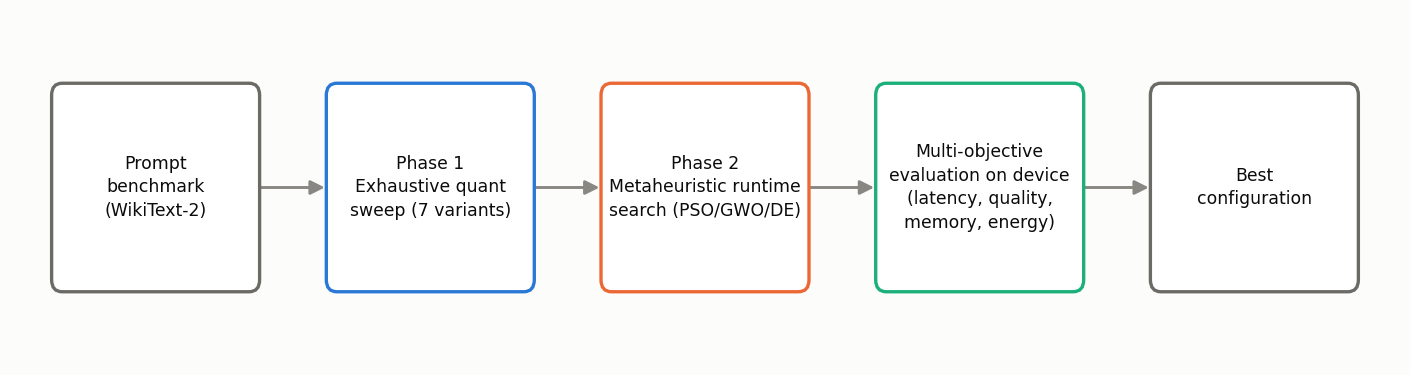
\includegraphics[width=\linewidth]{pipeline_diagram.png}
\caption{Overall two-phase pipeline: exhaustive Phase 1 sweep over quantization variants, followed by Phase 2's metaheuristic runtime-parameter search, both evaluated on-device against the joint objective (Section~\ref{sec:objective}).}
\label{fig:pipeline}
\end{figure}

\subsection{Target Platform, Benchmark, and Search Spaces}
\label{sec:phase1}
Target hardware is a Raspberry Pi 5 (8 GB RAM, Broadcom BCM2712, 4 Cortex-A76 cores, active PWM-fan cooling), Debian 13, llama.cpp built from source, CPU governor fixed to \texttt{performance}. Model is TinyLlama-1.1B-Chat-v1.0~\cite{ref1}; no pre-converted F16 GGUF was available, so Q8\_0 is used as the requantization source for all Phase 1 variants (a documented deviation, not true F16). Latency/throughput uses \texttt{llama-bench} (512 prompt / 128 generation tokens, 3 repetitions for Phase 1; Phase 2 varies prompt tokens directly as the searched $n_{\text{ctx}}$); quality uses \texttt{llama-perplexity} over WikiText-2.

Phase 1 candidates are the GGUF variants Q2\_K, Q3\_K\_M, Q4\_0, Q4\_K\_M, Q5\_K\_M, Q6\_K, Q8\_0; each is evaluated once for perplexity, peak RSS, tokens/second, and file size (Table~\ref{tab:phase1-impact}), and all variants not Pareto-dominated on (quality, memory, speed) are retained for Phase 2---no fixed top-$k$ cap.

Phase 2 searches a 4-dimensional mixed integer/categorical vector per retained variant (Table~\ref{tab:runtime-params}), encoded as a continuous box in $\mathbb{R}^4$ so PSO/GWO/DE never need to know the space is anything but continuous. $n_{\text{ctx}}$'s upper bound was capped at 1024 (not an originally planned 2048) after direct measurement showed larger prompt sizes cost real additional minutes per evaluation. Temperature and top-p were dropped from the search: they only affect quality through sampling randomness, which perplexity cannot distinguish.

\begin{table}[t]
\caption{Phase 2 runtime hyperparameter search space}
\label{tab:runtime-params}
\centering
\footnotesize
\begin{tabular}{@{}p{1.6cm}p{1.0cm}p{1.3cm}p{2.2cm}@{}}
\toprule
Parameter & Type & Range & Notes \\
\midrule
Threads & Integer & $[1,4]$ & Pi 5, 4 Cortex-A76 cores \\
Batch size (\texttt{n\_batch}) & Integer & $[32,512]$ & \texttt{-b} flag \\
Context length (\texttt{n\_ctx}) & Integer & $[128,1024]$ & via \texttt{-p} \\
KV-cache type & Categorical & \{f16, q8\_0, q4\_0\} & \texttt{-ctk}/\texttt{-ctv} \\
\bottomrule
\end{tabular}
\end{table}

\subsection{Objective Function}
\label{sec:objective}
We minimize a scalarized, constrained multi-objective function:
\begin{equation}
\label{eq:objective}
f(\mathbf{x}) = \alpha\,\hat{L}(\mathbf{x}) + \beta\,\bigl(1-\hat{Q}(\mathbf{x})\bigr) + \gamma\,\hat{M}(\mathbf{x}) + \delta\,\hat{E}(\mathbf{x}) + \mathrm{Penalty}(\mathbf{x})
\end{equation}
where $\hat{L}$, $\hat{Q}$, $\hat{M}$, $\hat{E}$ are min--max normalized latency, quality, peak memory, and energy per token, and $\mathrm{Penalty}(\mathbf{x})=+\infty$ (hard reject, not a finite soft penalty) if peak RSS exceeds the RAM ceiling or the process crashes/OOMs/times out---a configuration that will actually OOM on this hardware must never be numerically outweighed by a good quality score. Weights $\alpha{=}0.35$, $\beta{=}0.35$, $\gamma{=}0.2$, $\delta{=}0.1$ are illustrative defaults, not tuned; Section~\ref{sec:best-configs}'s Grid-vs-DE energy/latency split on Q4\_K\_M shows the scalarization is doing real, non-trivial work, since different weights could plausibly favor Grid's low-energy point over DE's lower overall cost.

\subsection{Metaheuristics and Evaluation-Cost Argument}
\label{sec:cost-argument}
We use PSO~\cite{ref8}, GWO~\cite{ref9}, and DE~\cite{ref10} (Table~\ref{tab:meta-params} gives parameters), unchanged mechanically from~\cite{ref11}'s classical-ML setting---what changes is the cost of the fitness function. In~\cite{ref11}, one evaluation (fit + cross-validate a KNN/SVM) costs milliseconds, permitting population$\times$iteration budgets of thousands of evaluations. On the Pi 5, one Phase-2 evaluation measured 21--60 s depending on variant---three to four orders of magnitude slower. A flat search at~\cite{ref11}'s budget would require 17--33 hours of device time for a \emph{single} algorithm on a \emph{single} variant; this is why Phase 2 uses a deliberately time-boxed, per-variant-adaptive budget (population 4, iterations 5--8, 2 runs---an evaluation floor chosen to keep each algorithm within a 12-minute time box per variant, confirmed against real per-variant totals in Section~\ref{sec:phase2-convergence}).

Before trusting them on this real, noisy objective, PSO/GWO/DE are validated on three closed-form benchmark functions following~\cite{ref11}'s protocol (population 20, 200 iterations, 10 runs): Sphere (dim 10, unimodal), Goldstein--Price (dim 2, multimodal, global min. 3), and FindValues (dim 5, asymmetric-bounds squared-error function, global min. 0)---the closest synthetic proxy to the real Phase 2 objective. Grid search, random search, PSO, GWO, and DE are also compared on these functions at a matched budget of 4,000 evaluations, establishing the baseline implementations are correct before the real hardware experiment.

\subsection{Measurement and Baselines}
\label{sec:measurement-protocol}
Latency, quality, memory, and energy are all measured on physical hardware rather than simulated. Energy is measured via the Pi 5's on-board PMIC (\texttt{vcgencmd pmic\_read\_adc}, not external instrumentation): total power is the sum of $V\times I$ across all reported rails, sampled concurrently with each benchmark (1.0 s interval) and integrated over wall-clock generation time. Thermal throttling (\texttt{vcgencmd get\_throttled} bits set, SoC $\approx$83--84.5\textdegree C under sustained load) and OS/background jitter were observed but not actively mitigated in the originally reported run (\texttt{bench\_repetitions=1}, one measurement per configuration, not repetition-averaged)---both are disclosed as limitations (Section~\ref{sec:limitations}) and directly motivate the hardened follow-up (Section~\ref{sec:hardened-followup}). Grid search and random search, evaluation-budget-matched to the metaheuristics, are implemented as baselines to directly test whether metaheuristics outperform naive search under an equal budget---a claim that must not be assumed without a control.

\begin{table}[t]
\caption{Metaheuristic parameters for Phase 2 (real hardware run)}
\label{tab:meta-params}
\centering
\footnotesize
\begin{tabular}{@{}lcccl@{}}
\toprule
Algorithm & Pop. & Iter. & Runs & Key parameters \\
\midrule
PSO & 4 & 5--8 & 2 & $w{=}1.0$, $w_{\text{damp}}{=}0.99$, $c_1{=}c_2{=}2.0$ \\
GWO & 4 & 5--8 & 2 & $a$ linear decay $2\to0$ \\
DE  & 4 & 5--8 & 2 & $\beta_{min}{=}0.2$, $\beta_{max}{=}0.9$, $p_{CR}{=}0.1$ \\
\bottomrule
\end{tabular}
\end{table}

\section{Results and Discussion}
\label{sec:results}

\subsection{Phase 1: Quantization Variant Impact}
\label{sec:phase1-results}

\begin{table}[t]
\caption{Phase 1 quantization variant impact (real, Pi 5)}
\label{tab:phase1-impact}
\centering
\footnotesize
\begin{tabular}{@{}lccccc@{}}
\toprule
Variant & PPL & Peak RSS (MB) & Gen tok/s & Prompt tok/s & Size (MB) \\
\midrule
Q2\_K    & 28.8148 & 495.4  & 25.62 & 34.15  & 413.0 \\
Q3\_K\_M & 21.6011 & 793.4  & 19.18 & 34.47  & 523.9 \\
Q4\_0    & 20.6162 & 1197.7 & 18.06 & 116.85 & 608.2 \\
Q4\_K\_M & 20.4490 & 1257.2 & 17.02 & 70.59  & 637.8 \\
Q5\_K\_M & 20.1640 & 1465.9 & 14.38 & 60.73  & 746.7 \\
Q6\_K    & 20.0001 & 1687.6 & 12.26 & 61.31  & 862.5 \\
Q8\_0    & 19.9734 & 2180.6 & 8.47  & 54.97  & 1116.5 \\
\bottomrule
\end{tabular}
\end{table}

\textbf{All 7 variants are Pareto-nondominated, and that is itself a finding}: quality, speed, and memory trade off perfectly monotonically with quantization level (every step toward Q8\_0 strictly improves perplexity while strictly increasing memory and decreasing throughput, zero exceptions), so no variant beats another on every axis simultaneously. Marginal quality return shrinks sharply past Q4\_K\_M (20.62$\to$19.97 PPL, a 3.2\% gain, while RSS nearly doubles and speed drops by more than half)---a poor trade for most deployment goals. Because each Phase 2 evaluation costs real seconds (Section~\ref{sec:cost-argument}), the real search began on a 3-variant subset (Q2\_K, Q4\_K\_M, Q8\_0) and was extended to the remaining 4 (Q3\_K\_M, Q4\_0, Q5\_K\_M, Q6\_K) once the pipeline proved stable across an unattended overnight run; all 7 are complete below.

\subsection{Metaheuristic Validation and Baseline Rehearsal (Synthetic)}
\label{sec:validation-results}

All three optimizers reach values effectively indistinguishable from each function's known global minimum in their best run, confirming correct implementations before trusting them on the real objective. The comparative pattern echoes~\cite{ref11}: PSO is uniformly strong and low-variance across all three functions; GWO is the most fragile on the multimodal/asymmetric problems (its FindValues median is over 30 times worse than its best run, plateauing around iteration 30 while PSO/DE continue descending for 150+ more---consistent with premature convergence once its alpha/beta/delta leaders cluster); DE is competitive but slower to fully converge on Sphere and FindValues. This premature-convergence pattern reproduces on the real Phase 2 objective for some variants but not others (Section~\ref{sec:phase2-convergence}).

At a matched budget of 4,000 evaluations, grid search collapses on Sphere (dim 10): a shared-resolution grid can only afford 2 points per axis, so no grid point can land near the interior optimum (best cost 1000, exactly the corner-stuck value); random search does far better (median 50.63) but still loses by 8--11 orders of magnitude to any metaheuristic. On FindValues (dim 5, asymmetric bounds---the closest synthetic proxy to the real Phase 2 space), grid search's best (4554) is worse than random search's \emph{median} (1523)---a direct empirical warning against grid search on Phase 2's real, similarly asymmetric parameter space.

\subsection{Phase 2: Convergence}
\label{sec:phase2-convergence}

Figure~\ref{fig:phase2-convergence-all} plots median best-cost-so-far (2 runs) for PSO/GWO/DE across all 7 variants; Table~\ref{tab:phase2-convergence-summary} gives the median final-iteration cost. Patterns vary substantially by variant:

\begin{itemize}
  \item \textbf{Q4\_K\_M:} DE reaches the lowest median final cost (0.0603) and, in its best single run, the lowest cost of any algorithm on this variant (0.0205). GWO converges earliest but plateaus at a visibly worse cost---the same premature-convergence pattern flagged on the synthetic functions reproduces here.
  \item \textbf{Q2\_K:} GWO overtakes both PSO and DE by iteration 4 rather than plateauing early as on Q4\_K\_M---the premature-convergence hypothesis does \emph{not} generalize to this variant.
  \item \textbf{Q8\_0:} GWO again converges fastest and lowest, reproducing Q2\_K's pattern rather than Q4\_K\_M's plateau---GWO's behavior is variant-dependent, not fixed.
  \item \textbf{Q3\_K\_M:} DE starts and stays lowest, plateauing after iteration 1---later shown (Section~\ref{sec:best-configs}) to be the most extreme optimizer's-curse discrepancy in the whole dataset (61.5 times its recorded cost).
  \item \textbf{Q4\_0:} a much lower per-evaluation cost (20.7 s) let the adaptive budget allocate 8 iterations instead of the 5-iteration floor; all three algorithms show genuine gradual descent rather than an early plateau---also the variant with the most trustworthy recorded costs.
  \item \textbf{Q5\_K\_M:} GWO shows the clearest, most consistent descent; DE improves only modestly and stays highest throughout, the weakest DE convergence of any variant.
  \item \textbf{Q6\_K (final variant):} PSO converges earliest and most smoothly; DE again shows the weakest, latest convergence, dropping substantially only at the final iteration.
\end{itemize}

\begin{figure*}[t]
\centering
\begin{subfigure}{0.24\textwidth}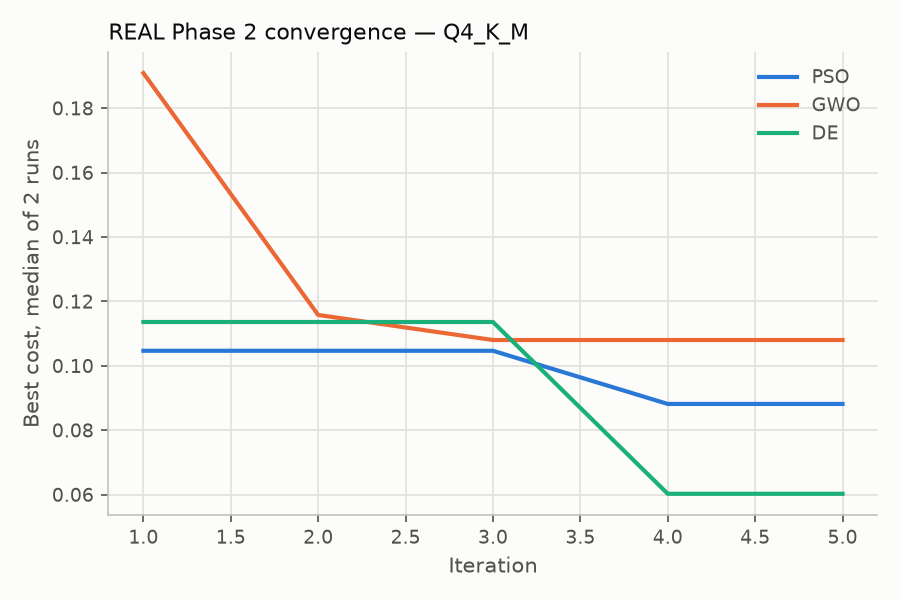
\includegraphics[width=\linewidth]{real_phase2_convergence_Q4_K_M.png}\caption{Q4\_K\_M}\end{subfigure}\hfill
\begin{subfigure}{0.24\textwidth}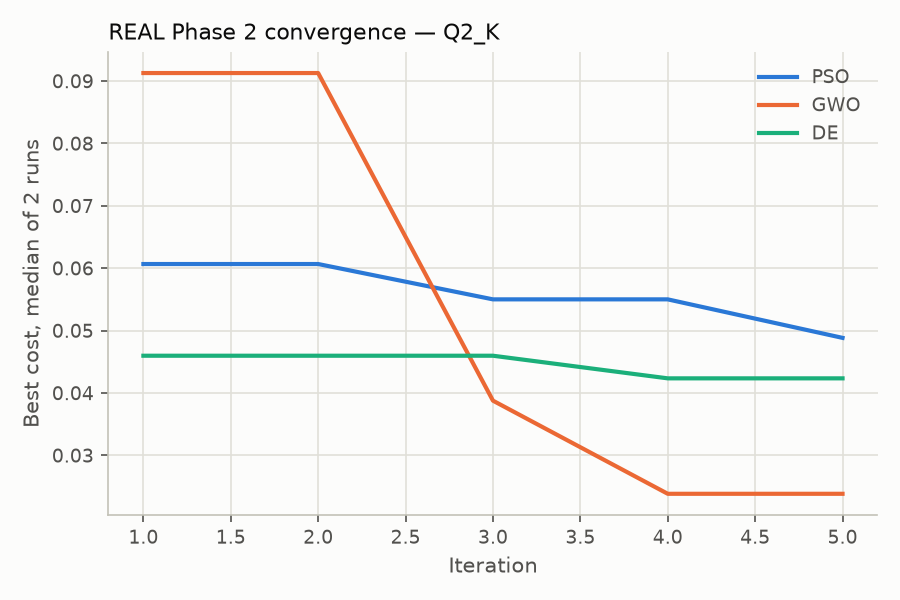
\includegraphics[width=\linewidth]{real_phase2_convergence_Q2_K.png}\caption{Q2\_K}\end{subfigure}\hfill
\begin{subfigure}{0.24\textwidth}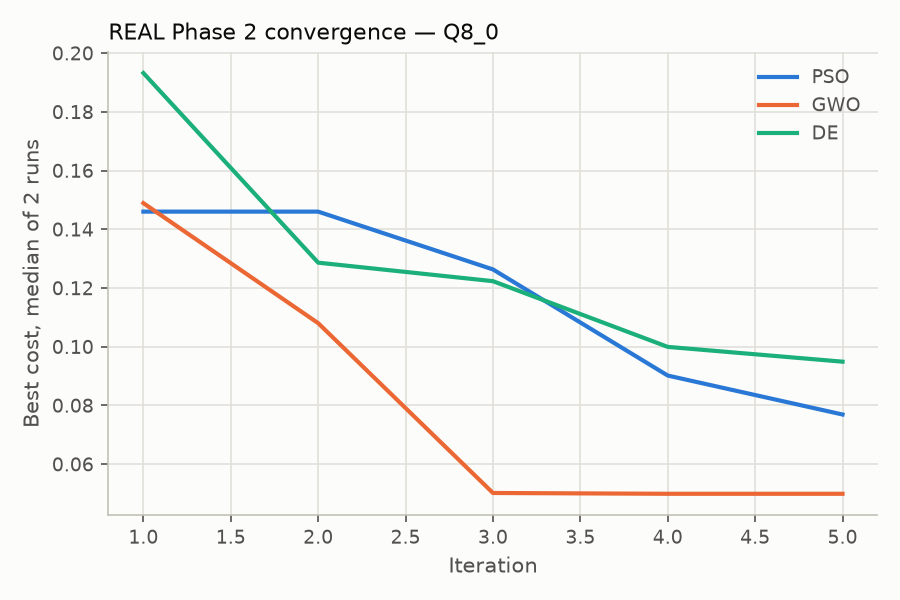
\includegraphics[width=\linewidth]{real_phase2_convergence_Q8_0.png}\caption{Q8\_0}\end{subfigure}\hfill
\begin{subfigure}{0.24\textwidth}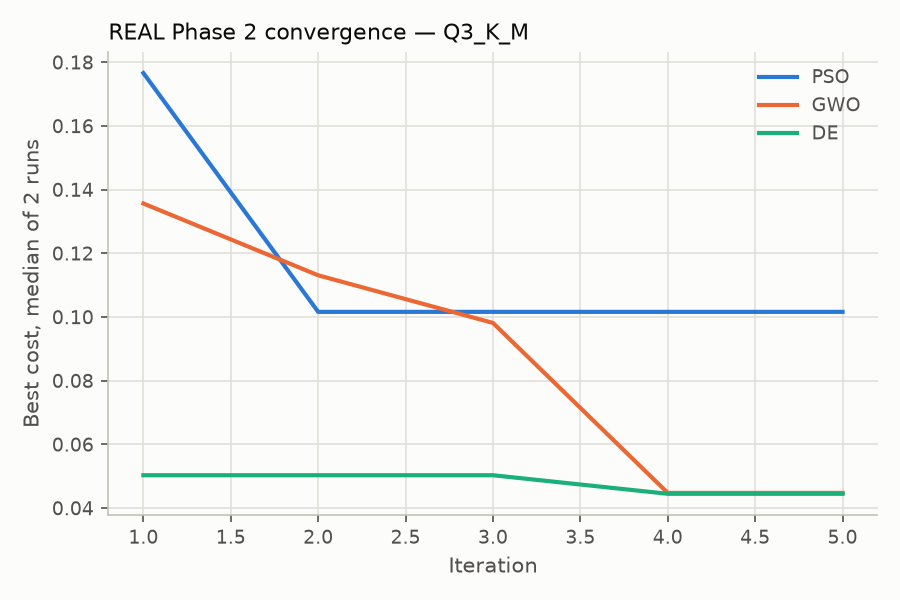
\includegraphics[width=\linewidth]{real_phase2_convergence_Q3_K_M.png}\caption{Q3\_K\_M}\end{subfigure}\\[4pt]
\begin{subfigure}{0.24\textwidth}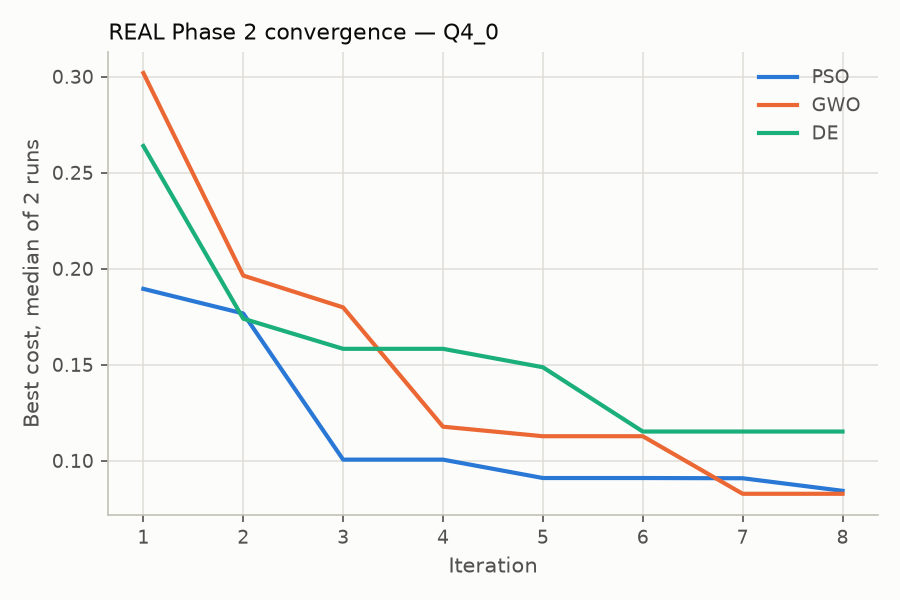
\includegraphics[width=\linewidth]{real_phase2_convergence_Q4_0.png}\caption{Q4\_0}\end{subfigure}\hfill
\begin{subfigure}{0.24\textwidth}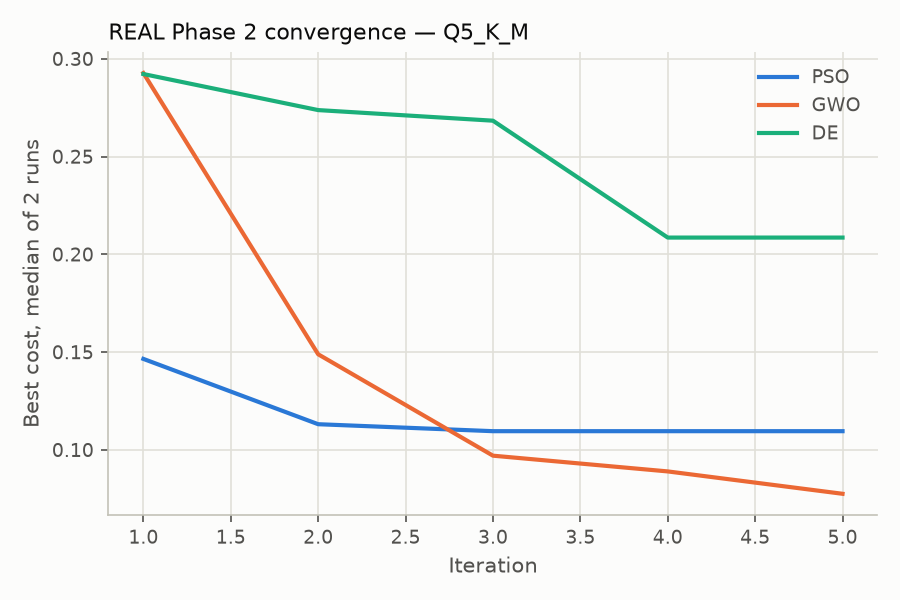
\includegraphics[width=\linewidth]{real_phase2_convergence_Q5_K_M.png}\caption{Q5\_K\_M}\end{subfigure}\hfill
\begin{subfigure}{0.24\textwidth}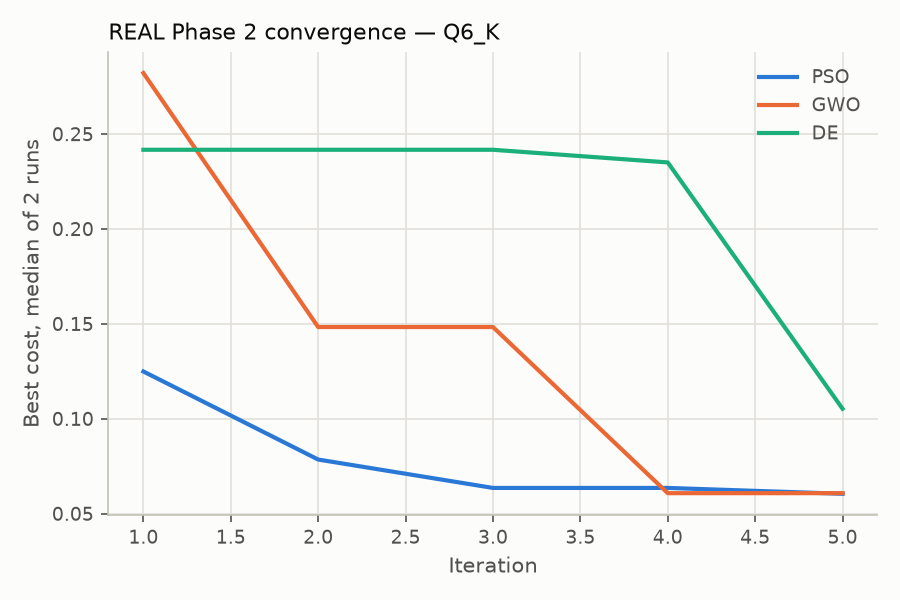
\includegraphics[width=\linewidth]{real_phase2_convergence_Q6_K.png}\caption{Q6\_K}\end{subfigure}
\caption{Real Phase 2 convergence, all 7 completed variants (median of 2 runs).}
\label{fig:phase2-convergence-all}
\end{figure*}

\begin{table}[t]
\caption{Real Phase 2 convergence summary --- median best cost of 2 runs at the final iteration, all 7 variants}
\label{tab:phase2-convergence-summary}
\centering
\footnotesize
\begin{tabular}{@{}lccccc@{}}
\toprule
Variant & Iters & PSO & GWO & DE & Per-eval (s) \\
\midrule
Q4\_K\_M & 5 & 0.0882 & 0.1080 & 0.0603 & 32.9 \\
Q2\_K    & 5 & 0.0488 & 0.0238 & 0.0423 & 59.9 \\
Q8\_0    & 5 & 0.0769 & 0.0499 & 0.0949 & 33.6 \\
Q3\_K\_M & 5 & 0.1016 & 0.0448 & 0.0445 & 51.0 \\
Q4\_0    & 8 & 0.0843 & 0.0828 & 0.1152 & 20.7 \\
Q5\_K\_M & 5 & 0.1095 & 0.0775 & 0.2086 & 35.0 \\
Q6\_K    & 5 & 0.0604 & 0.0608 & 0.1053 & 35.5 \\
\bottomrule
\end{tabular}
\end{table}

\subsection{Phase 2: Robustness Across Repeated Runs}
\label{sec:robustness}

Figure~\ref{fig:phase2-robustness-all} and Table~\ref{tab:phase2-robustness-summary} give per-run best cost. With $N_{\text{runs}}=2$---reduced from the synthetic-validation protocol's 10 because each run here costs real Pi wall-clock time---variance can only be characterized coarsely (Section~\ref{sec:limitations}):

\begin{itemize}
  \item \textbf{Q4\_K\_M:} the pattern \emph{inverts} synthetic-validation expectations---GWO, flagged as fragile on synthetic functions, is by far the \emph{most} consistent here (1.03 times spread) while PSO and DE swing 4--5 times between runs.
  \item \textbf{Q2\_K:} GWO's run 1 lands on a cost of \emph{exactly} 0.0000---every normalized term simultaneously at its clipped floor, a direct consequence of the small calibration sample ($N_{\text{calib}}=8$) rather than a true global optimum; Grid independently hit the same corner.
  \item \textbf{Q8\_0:} GWO's near-zero (0.0010) reveals a different issue---recomputing its cost from its own raw metrics gives $\approx$0.18, not 0.0010, pure single-measurement noise between the search-time and report-time evaluation of the same configuration.
  \item \textbf{Q3\_K\_M:} DE's run 1 (0.0026) is the overall best recorded cost across all 7 variants, and (per Section~\ref{sec:best-configs}) also the single most extreme optimizer's-curse discrepancy in the dataset; run 2 (0.0864) is unremarkable, flagging run 1 as the outlier.
  \item \textbf{Q4\_0:} the same outlier pattern recurs (GWO run 1 $\ll$ run 2), but this is the one variant where even the low outlier run is largely corroborated by its own raw metrics---consistent with its longer 8-iteration budget.
  \item \textbf{Q5\_K\_M:} GWO's run 1 (0.0073) is again a large outlier; DE's run 2 (0.3491) is notably the \emph{worst} single run recorded anywhere in this study.
  \item \textbf{Q6\_K:} all three algorithms show a broadly similar 3.5--6.2 times spread, without the extreme ($>$10 times) outliers seen on Q8\_0, Q3\_K\_M, and Q5\_K\_M---the most ``ordinary'' robustness profile of any variant.
\end{itemize}

\begin{figure*}[t]
\centering
\begin{subfigure}{0.24\textwidth}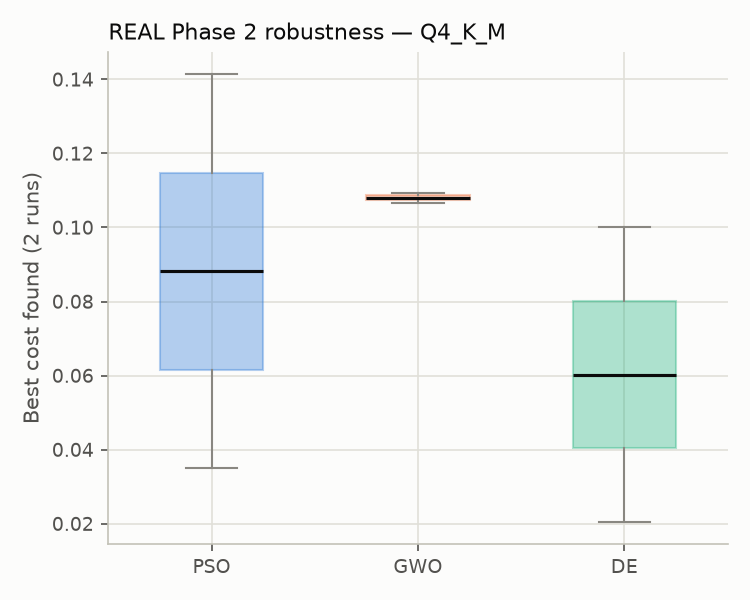
\includegraphics[width=\linewidth]{real_phase2_boxplot_Q4_K_M.png}\caption{Q4\_K\_M}\end{subfigure}\hfill
\begin{subfigure}{0.24\textwidth}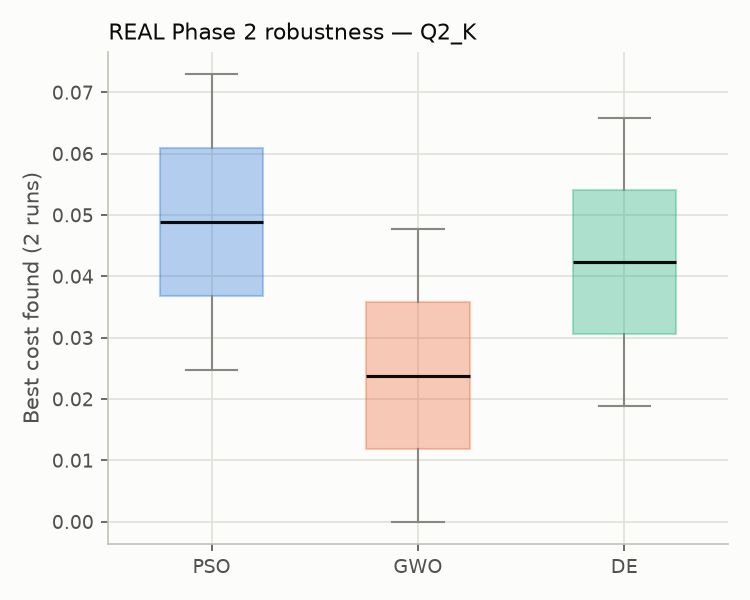
\includegraphics[width=\linewidth]{real_phase2_boxplot_Q2_K.png}\caption{Q2\_K}\end{subfigure}\hfill
\begin{subfigure}{0.24\textwidth}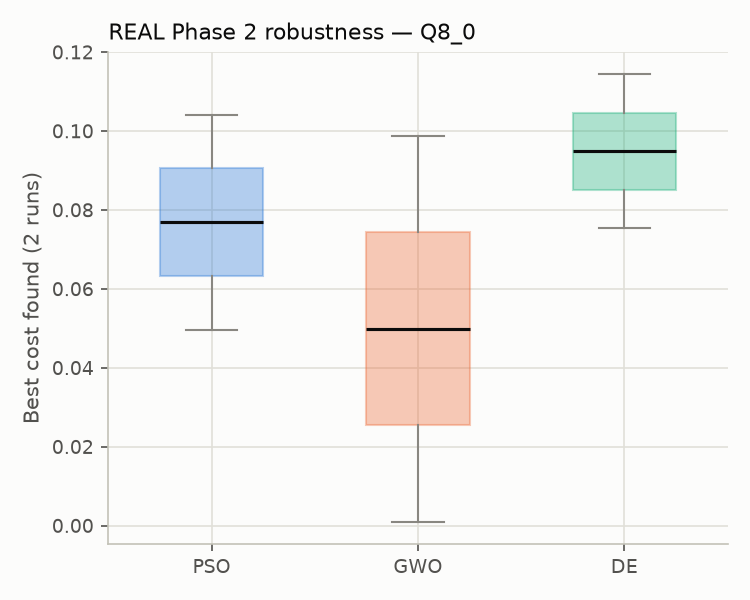
\includegraphics[width=\linewidth]{real_phase2_boxplot_Q8_0.png}\caption{Q8\_0}\end{subfigure}\hfill
\begin{subfigure}{0.24\textwidth}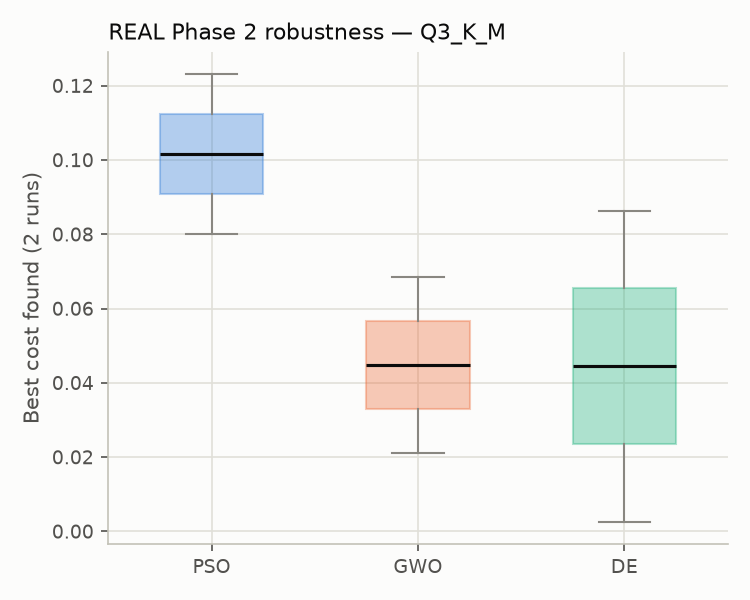
\includegraphics[width=\linewidth]{real_phase2_boxplot_Q3_K_M.png}\caption{Q3\_K\_M}\end{subfigure}\\[4pt]
\begin{subfigure}{0.24\textwidth}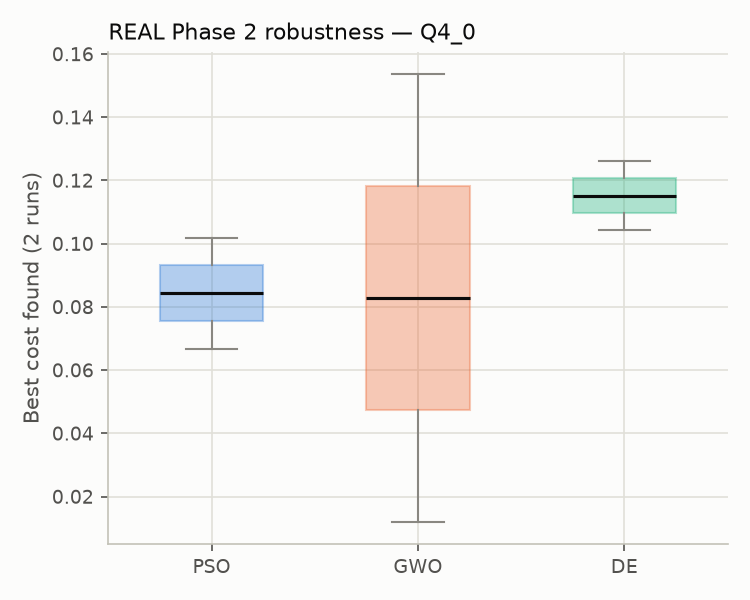
\includegraphics[width=\linewidth]{real_phase2_boxplot_Q4_0.png}\caption{Q4\_0}\end{subfigure}\hfill
\begin{subfigure}{0.24\textwidth}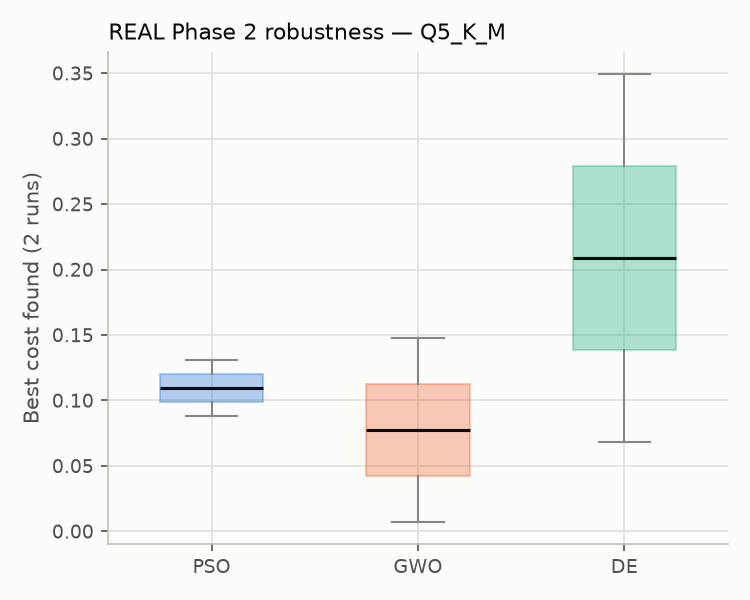
\includegraphics[width=\linewidth]{real_phase2_boxplot_Q5_K_M.png}\caption{Q5\_K\_M}\end{subfigure}\hfill
\begin{subfigure}{0.24\textwidth}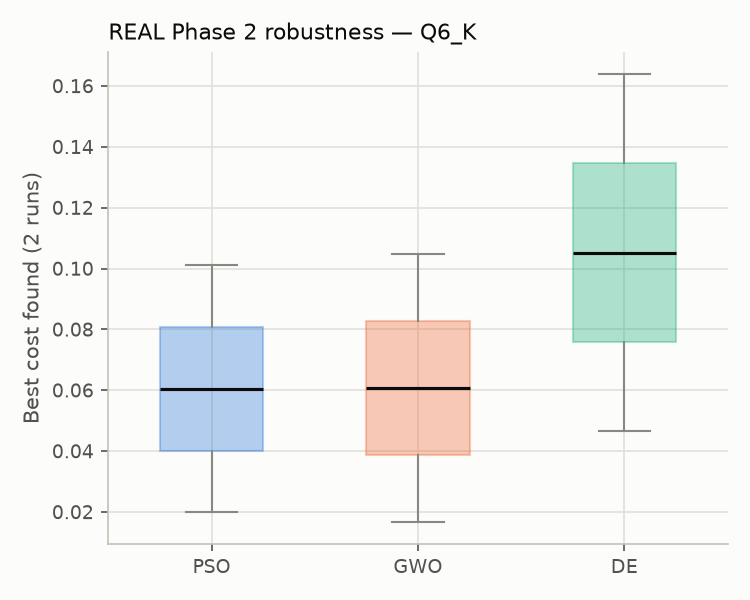
\includegraphics[width=\linewidth]{real_phase2_boxplot_Q6_K.png}\caption{Q6\_K}\end{subfigure}
\caption{Real Phase 2 robustness, all 7 completed variants (2 runs each).}
\label{fig:phase2-robustness-all}
\end{figure*}

\begin{table*}[t]
\caption{Per-run best cost and run-to-run spread, all 7 variants}
\label{tab:phase2-robustness-summary}
\centering
\footnotesize
\begin{tabular}{@{}lcccccccccc@{}}
\toprule
& \multicolumn{3}{c}{PSO} & \multicolumn{3}{c}{GWO} & \multicolumn{3}{c}{DE} \\
\cmidrule(lr){2-4}\cmidrule(lr){5-7}\cmidrule(lr){8-10}
Variant & Run 1 & Run 2 & Spread & Run 1 & Run 2 & Spread & Run 1 & Run 2 & Spread \\
\midrule
Q4\_K\_M & 0.0350 & 0.1414 & 4.0$\times$ & 0.1094 & 0.1066 & 1.03$\times$ & \textbf{0.0205} & 0.1000 & 4.9$\times$ \\
Q2\_K    & 0.0247 & 0.0729 & 3.0$\times$ & \textbf{0.0000} & 0.0477 & n/a (floor) & 0.0189 & 0.0658 & 3.5$\times$ \\
Q8\_0    & 0.0497 & 0.1042 & 2.1$\times$ & \textbf{0.0010} & 0.0988 & 99$\times$ & 0.1144 & 0.0755 & 1.5$\times$ \\
Q3\_K\_M & 0.1231 & 0.0802 & 1.5$\times$ & 0.0210 & 0.0685 & 3.3$\times$ & \textbf{0.0026} & 0.0864 & 33$\times$ \\
Q4\_0    & 0.0667 & 0.1019 & 1.5$\times$ & 0.0120 & 0.1536 & 12.8$\times$ & 0.1262 & 0.1043 & 1.2$\times$ \\
Q5\_K\_M & 0.0878 & 0.1312 & 1.5$\times$ & \textbf{0.0073} & 0.1477 & 20.2$\times$ & 0.0680 & 0.3491 & 5.1$\times$ \\
Q6\_K    & 0.0198 & 0.1011 & 5.1$\times$ & \textbf{0.0168} & 0.1048 & 6.2$\times$ & 0.0467 & 0.1638 & 3.5$\times$ \\
\bottomrule
\end{tabular}
\end{table*}

\subsection{The Optimizer's Curse: Best Configurations and Reconciliation}
\label{sec:best-configs}

Q2\_K's exact-zero GWO cost and Q8\_0's near-zero GWO cost prompted a systematic check, run across all 7 variants: recompute each method's scalarized cost from its own reported raw metrics (\texttt{best\_configs.csv}, run through the objective's actual weights and calibrated ranges) and compare against the recorded search-time cost (Table~\ref{tab:reconciliation}).

\begin{table}[t]
\caption{Reconstructed-cost / recorded-cost ratio, all 7 variants}
\label{tab:reconciliation}
\centering
\footnotesize
\begin{threeparttable}
\begin{tabular}{@{}lccccc@{}}
\toprule
Variant & PSO & GWO & DE & Random & Grid \\
\midrule
Q2\_K    & 0.00$\times$\tnote{c} & $\infty$\tnote{c} & 0.00$\times$\tnote{c} & 1.01$\times$ & $\infty$\tnote{c} \\
Q3\_K\_M & 2.89$\times$ & 8.45$\times$ & 61.51$\times$ & 2.60$\times$ & 0.93$\times$ \\
Q4\_0    & 0.89$\times$ & 1.16$\times$ & 1.02$\times$ & 1.33$\times$ & 1.00$\times$ \\
Q4\_K\_M & 6.06$\times$ & 1.98$\times$ & 7.01$\times$ & 0.96$\times$ & 0.80$\times$ \\
Q5\_K\_M & 1.40$\times$ & 22.50$\times$ & 1.54$\times$ & 2.91$\times$ & 1.32$\times$ \\
Q6\_K    & 0.72$\times$ & 1.12$\times$ & 0.00$\times$\tnote{c} & 0.20$\times$ & 1.33$\times$ \\
Q8\_0    & 1.14$\times$ & 179.89$\times$ & 3.16$\times$ & 2.33$\times$ & 8.20$\times$ \\
\bottomrule
\end{tabular}
\begin{tablenotes}
\item[c] {\scriptsize both values round to the calibration floor of 0.}
\end{tablenotes}
\end{threeparttable}
\end{table}

The pattern is consistent with the \textbf{optimizer's curse}: a population-based metaheuristic's iterative convergence toward a promising region repeatedly samples nearby-but-distinct configurations there, and the single lowest cost observed across those noisy real-hardware evaluations is a biased, overly optimistic estimator of that configuration's \emph{true} cost. Grid and Random search are far less exposed (ratios mostly near 1$\times$) because they do not iteratively concentrate sampling around a converging optimum---every ratio above 8$\times$ anywhere in this dataset belongs to a metaheuristic, never to Grid or Random. The recorded cost remains a fair basis for ranking methods against each other within a variant, but the raw-metric columns come from a separate, later re-evaluation and should be read as illustrative of the plausible trade-off space, not confirmed causal fact.

Table~\ref{tab:best-configs-all} gives the best configuration found by each method for every variant with its full raw re-measurement. \textbf{Bold} marks this paper's best-supported recommendation per variant; \textdagger\ marks a row excluded because its recorded cost does not reconcile with its own raw metrics.

\begin{itemize}
  \item \textbf{Q4\_K\_M:} the overall winner (DE) and second-best (PSO) agree closely on threads (3, not the maximum 4) and n\_batch ($\approx$310--320), differing mainly in n\_ctx and KV-cache type; DE's raw metrics reconstruct to 7.0$\times$ its recorded cost though, so its ``wins on energy'' story is illustrative, not confirmed. Grid's more reconcilable row (0.80$\times$) genuinely trades the smallest n\_ctx and lowest energy for the worst latency.
  \item \textbf{Q2\_K:} every method's best configuration uses threads=4, kv\_cache\_type=f16; PSO/GWO/DE/Grid all reconstruct to a clipped $\sim$0 cost, so this dataset cannot reliably rank them against each other---only Random's number is trustworthy, and it is also the worst of the five.
  \item \textbf{Q3\_K\_M:} DE's recorded win (0.0026) is the lowest cost anywhere in the dataset, but per its 61.5$\times$ reconciliation ratio this is the \emph{least} trustworthy single number in the entire study; Grid's genuinely reconcilable 0.1596 is arguably a more honest ``known'' number here.
  \item \textbf{Q4\_0:} because these numbers are trustworthy, a real mechanistic story can be told with confidence: GWO's win comes from threads=2 (not the maximum 4) with low peak memory and energy (0.964 J/tok); Grid's threads=1 corner is unambiguously the worst method here.
  \item \textbf{Q5\_K\_M:} excluding GWO's unreliable 0.0073, \textbf{Random search (0.0157) is actually the lowest recorded cost}, beating every metaheuristic---the second variant (after Q8\_0) where a naive baseline wins once the least-reliable number is set aside.
  \item \textbf{Q6\_K:} GWO's win (ratio 1.12$\times$, trustworthy) is genuinely the best-supported result on this variant, closely followed by PSO (ratio 0.72$\times$, also trustworthy)---a real, if narrow, GWO-over-PSO finding rather than noise.
  \item \textbf{Q8\_0:} \textbf{Taking Grid's 0.0239 as the real best result is the more defensible reading}, and it is genuinely uncomfortable for this paper's central claim: naive grid search outperforms two of the three metaheuristics on this largest, most expensive variant.
\end{itemize}

\begin{table*}[t]
\caption{Best configurations found, all 7 variants (raw re-measurement of each method's search-time winner)}
\label{tab:best-configs-all}
\centering
\scriptsize
\begin{tabular}{@{}llccccccccc@{}}
\toprule
Variant & Method & Threads & Batch & Ctx & KV & $f(x)$ & Latency (ms/tok) & Quality ($-$PPL) & Peak RSS (MB) & Energy (J/tok) \\
\midrule
Q2\_K & \textbf{GWO} & 4 & 153 & 128 & f16 & \textbf{0.0000} & 42.99 & $-$31.3272 & 468.8 & 1.257 \\
Q2\_K & Grid & 4 & 512 & 128 & f16 & 0.0000 & 44.83 & $-$31.3272 & 468.0 & 1.193 \\
Q2\_K & DE & 4 & 167 & 387 & f16 & 0.0189 & 42.83 & $-$31.3272 & 467.9 & 3.052 \\
Q2\_K & PSO & 4 & 221 & 409 & f16 & 0.0247 & 42.54 & $-$31.3272 & 468.9 & 3.173 \\
Q2\_K & Random & 4 & 318 & 387 & f16 & 0.0482 & 44.01 & $-$31.3272 & 476.9 & 3.158 \\
\addlinespace
Q3\_K\_M & \textbf{DE} & 4 & 228 & 128 & f16  & \textbf{0.0026} & 49.27 & $-$23.2585 & 785.7 & 1.115 \\
Q3\_K\_M & GWO & 4 & 244 & 465 & f16  & 0.0210 & 49.77 & $-$23.2585 & 785.3 & 3.269 \\
Q3\_K\_M & PSO & 4 & 205 & 831 & q8\_0 & 0.0802 & 49.61 & $-$23.2639 & 784.2 & 6.250 \\
Q3\_K\_M & Random & 4 & 273 & 819 & q8\_0 & 0.1049 & 51.07 & $-$23.2639 & 784.6 & 6.308 \\
Q3\_K\_M & Grid & 4 & 32 & 128 & f16  & 0.1596 & 49.12 & $-$23.2585 & 784.5 & 1.138 \\
\addlinespace
Q4\_0 & \textbf{GWO} & 2 & 179 & 294 & q8\_0 & \textbf{0.0120} & 48.83 & $-$22.3364 & 1159.5 & 0.964 \\
Q4\_0 & Random & 2 & 181 & 182 & f16 & 0.0157 & 48.57 & $-$22.3562 & 1160.6 & 0.663 \\
Q4\_0 & PSO & 2 & 299 & 380 & q8\_0 & 0.0667 & 48.70 & $-$22.3364 & 1170.0 & 1.238 \\
Q4\_0 & DE & 2 & 47 & 930 & q8\_0 & 0.1043 & 48.62 & $-$22.3364 & 1154.1 & 3.564 \\
Q4\_0 & Grid & 1 & 32 & 128 & f16 & 0.3098 & 57.03 & $-$22.3562 & 1146.4 & 0.718 \\
\addlinespace
Q4\_K\_M & \textbf{DE}    & 3 & 318 & 387 & f16  & \textbf{0.0205} & 53.86 & $-$22.3879 & 1248.5 & 1.639 \\
Q4\_K\_M & PSO   & 3 & 308 & 567 & q8\_0 & 0.0350 & 54.61 & $-$22.3722 & 1252.5 & 2.689 \\
Q4\_K\_M & GWO   & 3 & 217 & 764 & q8\_0 & 0.1066 & 54.97 & $-$22.3722 & 1249.6 & 3.568 \\
Q4\_K\_M & Random & 3 & 311 & 663 & f16  & 0.1238 & 54.65 & $-$22.3879 & 1243.7 & 2.725 \\
Q4\_K\_M & Grid  & 4 & 512 & 128 & f16  & 0.3311 & 63.02 & $-$22.3879 & 1239.5 & 0.805 \\
\addlinespace
Q5\_K\_M & GWO\textdagger & 3 & 313 & 323 & f16 & \emph{0.0073} & 64.19 & $-$21.9608 & 1451.0 & 1.731 \\
Q5\_K\_M & DE & 3 & 167 & 387 & f16 & 0.0680 & 63.17 & $-$21.9608 & 1450.8 & 2.086 \\
Q5\_K\_M & PSO & 3 & 310 & 697 & q8\_0 & 0.0878 & 62.52 & $-$21.9742 & 1449.2 & 3.753 \\
Q5\_K\_M & \textbf{Random} & 3 & 66 & 419 & f16 & \textbf{0.0157} & 62.30 & $-$21.9608 & 1449.6 & 2.232 \\
Q5\_K\_M & Grid & 4 & 32 & 128 & f16 & 0.2486 & 67.22 & $-$21.9608 & 1450.4 & 0.936 \\
\addlinespace
Q6\_K & \textbf{GWO} & 3 & 202 & 359 & f16 & \textbf{0.0168} & 72.96 & $-$21.7199 & 1669.2 & 2.076 \\
Q6\_K & PSO & 3 & 309 & 455 & f16 & 0.0198 & 72.92 & $-$21.7199 & 1668.1 & 2.382 \\
Q6\_K & Random & 3 & 66 & 419 & f16 & 0.0371 & 72.87 & $-$21.7199 & 1667.0 & 2.355 \\
Q6\_K & DE & 3 & 48 & 387 & f16 & 0.0467 & 72.65 & $-$21.7199 & 1664.6 & 2.059 \\
Q6\_K & Grid & 4 & 32 & 128 & f16 & 0.2455 & 77.80 & $-$21.7199 & 1671.1 & 1.163 \\
\addlinespace
Q8\_0 & GWO\textdagger & 2 & 108 & 128 & f16 & \emph{0.0010} & 85.86 & $-$21.7013 & 2179.6 & 0.841 \\
Q8\_0 & \textbf{Grid} & 1 & 32  & 128 & f16 & \textbf{0.0239} & 87.51 & $-$21.7013 & 2179.3 & 0.987 \\
Q8\_0 & Random & 2 & 95  & 688 & f16 & 0.0340 & 86.04 & $-$21.7013 & 2164.8 & 2.916 \\
Q8\_0 & PSO    & 2 & 279 & 797 & f16 & 0.0497 & 86.08 & $-$21.7013 & 2161.0 & 3.218 \\
Q8\_0 & DE     & 2 & 47  & 867 & f16 & 0.0755 & 85.75 & $-$21.7013 & 2177.9 & 4.009 \\
\bottomrule
\end{tabular}
\end{table*}

\subsection{Comparison Against Baselines}
\label{sec:baseline-comparison-real}

At the matched evaluation budget (population 4 $\times$ iterations 5 = 20 evaluations for PSO/GWO/DE and Random), the metaheuristic-vs-baseline margin varies as sharply across variants as the reconciliation ratios above:

\begin{itemize}
  \item \textbf{Q4\_K\_M:} all three metaheuristics beat both naive baselines; DE beats grid search by 16.1$\times$ and random search by 6.0$\times$---the clean version of this paper's central motivating claim.
  \item \textbf{Q2\_K:} \textbf{complicates} that clean narrative: grid \emph{ties} the best metaheuristic only because both land on the same under-calibrated corner; the dataset does not support a specific numeric margin for this variant at all.
  \item \textbf{Q3\_K\_M:} naively read, DE beats grid by 61$\times$---the largest margin in the study---but that number is also the least trustworthy result in the whole dataset, so it should not be reported at face value.
  \item \textbf{Q4\_0:} the one variant where the margin is fully trustworthy: GWO beats grid by 25.8$\times$ and random by 1.3$\times$; all three metaheuristics beat grid decisively.
  \item \textbf{Q5\_K\_M:} excluding GWO, \textbf{random search wins outright}, beating every metaheuristic including the best reasonably-trustworthy one (DE, 4.3$\times$ worse).
  \item \textbf{Q6\_K:} a clean metaheuristic win returns: GWO beats grid by 14.6$\times$ and random by 2.2$\times$, corroborated by reasonably close reconciliation ratios.
  \item \textbf{Q8\_0:} excluding GWO's unreliable number, \textbf{grid search wins}, beating PSO by 2.1$\times$ and DE by 3.2$\times$---the opposite of Q4\_K\_M's result.
\end{itemize}

\subsection{Discussion}
\label{sec:discussion}

\begin{table}[t]
\caption{Cross-variant summary}
\label{tab:cross-variant-summary}
\centering
\footnotesize
\begin{tabular}{@{}lp{2.2cm}p{1.8cm}p{1.5cm}@{}}
\toprule
Variant & Best trustworthy method & Margin over grid & Reconciliation \\
\midrule
Q4\_K\_M & DE (ratio 7.0$\times$, weak) & 16.1$\times$ recorded, not fully trustworthy & poor \\
Q2\_K & unresolved & not numerically resolvable & poor (4/5 clipped) \\
Q3\_K\_M & DE recorded win, ratio 61.5$\times$ (worst) & $\sim$61$\times$ recorded; do not trust & very poor \\
Q4\_0 & GWO, ratio 1.16$\times$ & 25.8$\times$, trustworthy & \textbf{excellent} \\
Q5\_K\_M & Random search wins over all metaheuristics & --- (baseline wins) & Random/DE/Grid fair; GWO 22.5$\times$ \\
Q6\_K & GWO, ratio 1.12$\times$ & 14.6$\times$, trustworthy & good \\
Q8\_0 & Grid itself wins & --- & Grid fair; GWO 180$\times$ \\
\bottomrule
\end{tabular}
\end{table}

\textbf{The paper's central empirical finding, supported by all 7 variants, is not ``how much do metaheuristics beat baselines'' but ``how reliably can this be measured at all''}---and the answer depends heavily on per-variant noise conditions that the two-phase design surfaces rather than averages away. Two variants give fully trustworthy metaheuristic wins; two see a naive baseline outright beat every metaheuristic once unreliable numbers are excluded; the remaining three range from partially confounded to actively misleading if taken at face value. This is, to our knowledge, the first concrete, measured account of the optimizer's curse as a failure mode specific to hardware-in-the-loop metaheuristic-tuned LLM deployment, rather than a generic risk asserted in the abstract. The mechanistic reason traces back to Section~\ref{sec:cost-argument}'s cost argument: real hardware evaluation is expensive, so Phase 2's necessarily small budget is far more exposed to per-variant noise, calibration undersampling, and the optimizer's curse than the millisecond-scale, thousands-of-evaluations budget used in synthetic validation or in~\cite{ref11}. A single quantization variant chosen up front, without the two-phase structure, would have reported only one of seven qualitatively different outcomes as if it were the general finding---the two-phase decomposition's full 7-variant coverage is what makes this cross-variant picture visible at all.

\subsection{Post-Experiment Verification (Hardened Follow-Up)}
\label{sec:hardened-followup}

To directly test whether the top future-work fix proposed above actually resolves the optimizer's curse rather than merely diagnosing it, the pipeline was hardened (\texttt{search\_bench\_repetitions}$=3$, an independent \texttt{verification\_bench\_repetitions}$=5$ re-measurement of each method's search-time winner, $N_{\text{calib}}=24$, a per-evaluation thermal gate, and crash-safe checkpointing) and re-run on 2026-09-07/08 on 4 of the 7 variants (Q3\_K\_M, Q4\_0, Q5\_K\_M, Q6\_K), writing to a separate results directory rather than overwriting the original data reported above.

\begin{table}[t]
\caption{Hardened follow-up: verified winners, 4 re-run variants}
\label{tab:hardened-followup}
\centering
\footnotesize
\begin{tabular}{@{}lcll@{}}
\toprule
Variant & Verified/5 & Winner & Cost (search$\to$verified) \\
\midrule
Q3\_K\_M & 2/5 & Random & 0.0522 $\to$ 0.0540 \\
Q4\_0    & 4/5 & PSO    & 0.0319 $\to$ 0.0349 \\
Q5\_K\_M & 0/5 & \textbf{none} & --- \\
Q6\_K    & 1/5 & Random & 0.0445 $\to$ 0.0570 \\
\bottomrule
\end{tabular}
\end{table}

The fix works as intended---it refuses to report a winner it cannot corroborate, rather than silently reporting an unreliable one---but it does not eliminate the underlying noise. Even after tripling search-time repetitions, GWO and DE remain ``unstable'' (fail the independent 5-repetition re-check) on 3 of the 4 re-run variants, confirming the original finding was not a single-measurement artifact. Two results go further than the original analysis: on \textbf{Q5\_K\_M}, \emph{no method reconciles, including both baselines}---the strongest evidence yet that this is a hardware-measurement-noise problem, not one confined to iteratively-converging methods. On \textbf{Q6\_K}, the original post-hoc check called GWO's win trustworthy (ratio 1.12$\times$, Table~\ref{tab:reconciliation}); under this stricter, independently re-measured bar, GWO's win does \emph{not} reconcile---a genuine correction, reported here rather than smoothed over. \textbf{Q4\_0} remains the best-behaved variant under both analyses (4 of 5 methods verified here), consistent with its longer 8-iteration search budget. Full per-method verification detail is in the repository (Section~\ref{sec:data-availability}).

\section{Limitations and Threats to Validity}
\label{sec:limitations}

\begin{itemize}
  \item \textbf{Single model family and hardware target}: TinyLlama-1.1B on Pi 5 only; generalization untested.
  \item \textbf{Scalarized objective with fixed, untuned weights} collapses a genuine multi-objective trade-off into one number; Section~\ref{sec:best-configs}'s Q4\_K\_M split (Grid wins on energy alone but loses overall) shows this is doing real work, not cosmetic aggregation. A Pareto-front analysis would be more informative but more expensive.
  \item \textbf{Small calibration sample} ($N_{\text{calib}}=8$) measurably changed a result: on Q2\_K, two independent optima landed outside the calibrated min/max window and clipped to an exact cost of 0.0000---a normalization artifact, not a true global optimum.
  \item \textbf{The optimizer's curse is general and pervasive}, not an isolated anomaly: \texttt{bench\_repetitions=1} means each evaluation is one noisy hardware measurement; reconstructing costs from raw metrics (Section~\ref{sec:best-configs}) disagrees with the recorded cost by up to 180$\times$, and every ratio above 8$\times$ belongs to a metaheuristic, never Grid/Random. A hardened follow-up (Section~\ref{sec:hardened-followup}) confirms this is not a single-measurement artifact and surfaces a stronger result: one re-run variant (Q5\_K\_M) reconciles for \emph{no} method at all, baselines included.
  \item \textbf{$N_{\text{runs}}$ reduced from 10 to 2} for real Phase 2: reported spread is the gap between two samples, not a statistically grounded estimate.
  \item \textbf{Hardware measurement noise} (thermal throttling at 83--84.5\textdegree C) may dominate small differences between top configurations; a mid-run Pi crash, likely thermal, lost no completed data but exposed the runner's lack of checkpoint/resume capability, since addressed (Section~\ref{sec:hardened-followup}).
  \item \textbf{Quality metric is perplexity, not task accuracy}, which is why temperature/top-p were dropped from the search space; a downstream task benchmark might rank configurations differently.
  \item \textbf{Novelty claim} rests on four targeted web-search passes, not a full database-backed citation-graph review; a Google Scholar/Semantic Scholar/Scopus traversal from~\cite{ref19,ref20,ref21,ref22} could still surface closer prior art.
\end{itemize}

\section{Conclusion and Future Work}
\label{sec:conclusion}

This paper set out to answer whether a two-phase decomposition---exhaustive discrete quantization selection followed by metaheuristic runtime tuning---is a feasible, worthwhile way to structure edge-LLM configuration search on physical hardware, and how PSO/GWO/DE compare for this task under real hardware-in-the-loop measurement rather than synthetic validation. Phase 1's exhaustive sweep found all 7 candidate variants Pareto-nondominated, and Phase 2's real search across all 7 retained variants showed that the best achievable configuration, its cost, and even \emph{how reliably that cost can be trusted at all} differ substantially by variant. A systematic reconciliation check---recomputing every reported ``best'' configuration's cost from an independent re-measurement---revealed the \textbf{optimizer's curse}: population-based metaheuristics' iterative convergence repeatedly samples near a promising region, so their reported best is a biased, overly optimistic estimator of true cost, far more so than grid or random search's more spread-out sampling. A hardened follow-up experiment then tested the obvious fix (repeated measurement plus independent verification) directly on hardware: it works as a safeguard---correctly withholding unreliable winners---but does not eliminate the underlying noise, and on one variant no method reconciles at all. This directly explains why a naive baseline outright wins on some variants and why one metaheuristic's apparent 61$\times$ margin should not be trusted: not because metaheuristics are worse optimizers, but because their own search dynamics expose their reported bests to a specific, nameable, now-measured statistical bias that cheap synthetic validation never surfaces. To our knowledge, this is the first time this failure mode has been concretely measured, and a proposed fix directly tested on hardware, for metaheuristic-tuned LLM deployment specifically.

Future work, in priority order: (1) extend the hardened follow-up to the remaining 3 variants for full 7/7 coverage, and investigate whether still-higher repetition counts or a fundamentally different measurement protocol (e.g., averaging across multiple thermal cycles) can resolve Q5\_K\_M-style variants where no method currently reconciles; (2) multi-objective Pareto-front search (NSGA-II/MOEA-D) instead of scalarization; (3) a downstream task-accuracy quality metric, reopening the temperature/top-p dimensions dropped here; (4) extension to other edge platforms and small models to test whether the variant-to-variant instability found here is hardware-specific or general; (5) hybrid metaheuristics and additional Phase 1 compression axes (structured pruning, LoRA-merged distillation).

\section*{Declarations}
\label{sec:data-availability}
\textbf{Data Availability:} Code, configuration, and all raw measurement data (Phase 1 sweep results, Phase 2 convergence/robustness/best-configuration CSVs, the Section~\ref{sec:hardened-followup} hardened follow-up data, and figures) referenced in this paper, including full repository structure and pseudocode, are maintained at \url{https://github.com/Koraiche/phd-hypetune-service}, currently a private repository that will be made public upon publication. The WikiText-2 corpus used for perplexity measurement is a standard, separately-licensed public dataset and is not redistributed in this repository. Funding, Author Contributions, and Conflict of Interest declarations are to be completed by the authors prior to submission.

\bibliographystyle{IEEEtran}
\begin{thebibliography}{99}

\bibitem{ref1} P. Zhang, G. Zeng, T. Wang, and W. Lu, ``TinyLlama: An Open-Source Small Language Model,'' \emph{arXiv:2401.02385}, 2024.

\bibitem{ref2} ggml-org, ``GGUF File Format Specification,'' \emph{ggml} [GitHub repository], \url{https://github.com/ggml-org/ggml/blob/master/docs/gguf.md}.

\bibitem{ref3} G. Gerganov et al., \emph{llama.cpp} [Software]. \url{https://github.com/ggml-org/llama.cpp}.

\bibitem{ref4} E. Frantar, S. Ashkboos, T. Hoefler, and D. Alistarh, ``GPTQ: Accurate Post-Training Quantization for Generative Pre-trained Transformers,'' \emph{arXiv:2210.17323}, 2022.

\bibitem{ref5} J. Lin, J. Tang, H. Tang, S. Yang, W.-M. Chen, W.-C. Wang, G. Xiao, X. Dang, C. Gan, and S. Han, ``AWQ: Activation-aware Weight Quantization for LLM Compression and Acceleration,'' \emph{arXiv:2306.00978}, 2023.

\bibitem{ref6} T. Dettmers, M. Lewis, Y. Belkada, and L. Zettlemoyer, ``LLM.int8(): 8-bit Matrix Multiplication for Transformers at Scale,'' \emph{arXiv:2208.07339}, 2022.

\bibitem{ref7} S. Kim, C. Hooper, A. Gholami, Z. Dong, X. Li, S. Shen, M. W. Mahoney, and K. Keutzer, ``SqueezeLLM: Dense-and-Sparse Quantization,'' \emph{arXiv:2306.07629}, 2023.

\bibitem{ref8} J. Kennedy and R. Eberhart, ``Particle swarm optimization,'' in \emph{Proc. ICNN'95 -- Int. Conf. Neural Networks}, vol. 4, 1995, pp. 1942--1948.

\bibitem{ref9} S. Mirjalili, S. M. Mirjalili, and A. Lewis, ``Grey wolf optimizer,'' \emph{Advances in Engineering Software}, vol. 69, pp. 46--61, 2014.

\bibitem{ref10} R. Storn and K. Price, ``Differential evolution -- a simple and efficient heuristic for global optimization over continuous spaces,'' \emph{Journal of Global Optimization}, vol. 11, no. 4, pp. 341--359, 1997.

\bibitem{ref11} Z. Nouna, H. Bouyghf, M. Nahid, and I. Sabiri, ``Heart disease prediction optimization using metaheuristic algorithms,'' \emph{IAES International Journal of Artificial Intelligence}, vol. 14, no. 5, pp. 4332--4341, 2025.

\bibitem{ref12} K. Wang, Z. Liu, Y. Lin, J. Lin, and S. Han, ``HAQ: Hardware-Aware Automated Quantization with Mixed Precision,'' in \emph{Proc. IEEE/CVF Conf. Computer Vision and Pattern Recognition (CVPR)}, 2019, pp.~8612--8620, doi: 10.1109/CVPR.2019.00881.

\bibitem{ref13} J. B. P. Matos Jr., I. Bessa, E. Manino, X. Song, and L. C. Cordeiro, ``CEG4N: Counter-Example Guided Neural Network Quantization Refinement,'' in \emph{Proc. Int. Workshop on Numerical Software Verification / Formal Methods for ML-Enabled Autonomous Systems (NSV/FoMLAS)}, Springer LNCS vol. 13466, 2022, pp.~29--45, doi: 10.1007/978-3-031-21222-2\_3.

\bibitem{ref14} P. Dong, L. Li, Z. Wei, X.-Y. Niu, Z. Tian, and H. Pan, ``EMQ: Evolving Training-free Proxies for Automated Mixed Precision Quantization,'' in \emph{Proc. IEEE/CVF Int. Conf. Computer Vision (ICCV)}, 2023.

\bibitem{ref15} J. Tmamna, E. Ben Ayed, and M. Ben Ayed, ``Automatic Quantization of Convolutional Neural Networks Based on Enhanced Bare-Bones Particle Swarm Optimization for Chest X-Ray Image Classification,'' in \emph{Computational Collective Intelligence (ICCCI 2023)}, Springer, 2023, pp.~125--137, doi: 10.1007/978-3-031-41456-5\_10.

\bibitem{ref16} S. Hameed, B. Qolomany, S. B. Belhaouari, M. Abdallah, J. Qadir, and A. Al-Fuqaha, ``Large Language Model Enhanced Particle Swarm Optimization for Hyperparameter Tuning for Deep Learning Models,'' \emph{arXiv:2504.14126}, 2025.

\bibitem{ref17} Y. Zheng, Y. Chen, B. Qian, X. Shi, Y. Shu, and J. Chen, ``A Review on Edge Large Language Models: Design, Execution, and Applications,'' \emph{ACM Computing Surveys}, vol. 57, no. 8, Art. 209, Mar. 2025.

\bibitem{ref18} D. Xu, H. Zhang, L. Yang, R. Liu, G. Huang, M. Xu, and X. Liu, ``Fast On-device LLM Inference with NPUs,'' in \emph{Proc. 30th ACM Int. Conf. on Architectural Support for Programming Languages and Operating Systems (ASPLOS)}, 2025.

\bibitem{ref19} M. Ardakani, J. Malekar, and R. Zand, ``LLMPi: Optimizing LLMs for High-Throughput on Raspberry Pi,'' in \emph{Proc. IEEE/CVF Conf. Computer Vision and Pattern Recognition Workshops (CVPRW), EDGE Workshop}, 2025, pp.~6379--6388.

\bibitem{ref20} A. A. Chowdhury, M. A. Hossen, M. A. Azam, and M. H. Rahman, ``DeepQGHO: Quantized Greedy Hyperparameter Optimization in Deep Neural Networks for On-the-Fly Learning,'' \emph{IEEE Access}, vol.~10, pp.~6407--6416, 2022.

\bibitem{ref21} Z. Zhang, A. Le Metzger, J. Lyu, C.-C. Chang, J. Shao, Y. Liu, E. A. Mensah, E. Wang, K. Heimerl, G. D. Abowd, S. Patel, N. Jaques, and V. Iyer, ``Embedded Arena: Iterative Optimization via Hardware Feedback,'' \emph{arXiv:2606.16190}, 2026.

\bibitem{ref22} S. Sadheerthan, M.-J. Hsu, C.-H. Huang, and Y.-T. Wang, ``Attention Distribution-Aware Softmax for NPU-Accelerated On-Device Inference of LLMs: An Edge-Oriented Approximation Design,'' \emph{Electronics}, vol.~15, no.~6, Art.~1312, 2026, doi: 10.3390/electronics15061312.

\end{thebibliography}

\appendix

\begin{algorithm}
\caption{Phase 1 --- Exhaustive quantization sweep}
\label{alg:phase1}
\begin{algorithmic}[1]
\For{variant $\in$ QUANT\_VARIANTS}
  \State load\_model(variant)
  \State result[variant] $\leftarrow$ evaluate(quality, memory, load\_time, speed)
\EndFor
\State retained $\leftarrow$ pareto\_nondominated(result, axes=\{quality, memory, speed\})
\end{algorithmic}
\end{algorithm}

\begin{algorithm}
\caption{Phase 2 --- Metaheuristic runtime search (per retained variant)}
\label{alg:phase2}
\begin{algorithmic}[1]
\For{variant $\in$ retained}
  \State load\_model(variant) \Comment{loaded once, reused across all evaluations}
  \For{algorithm $\in$ \{PSO, GWO, DE\}}
    \For{run $= 1$ to $N_{\mathrm{runs}}$}
      \State population $\leftarrow$ init\_population(RUNTIME\_PARAM\_SPACE)
      \For{iteration $= 1$ to $\mathrm{MAX\_ITER}$}
        \For{candidate $\in$ population}
          \If{infeasible(candidate)} \Comment{RAM ceiling, crash, timeout}
            \State fitness $\leftarrow +\infty$ \Comment{reject, no soft penalty}
          \Else
            \State fitness $\leftarrow f(\text{candidate})$ \Comment{Eq.~\eqref{eq:objective}, measured on device}
          \EndIf
        \EndFor
        \State update\_population(algorithm, population, fitness)
        \State log(best\_so\_far)
      \EndFor
      \State record(best\_of\_run)
    \EndFor
  \EndFor
\EndFor
\end{algorithmic}
\end{algorithm}

\end{document}
